% COSC 4P03 Project
% sudoku generator
% Taras Mychaskiw

\section{Introduction}

    \subsection{Terms}
    Here are the terms and names that will be used in this paper.
    \begin{center}\begin{tabular}{c||c}
        \hline
        $p$         &   the width of each box in the sudoku                             \\
        $q$         &   the height of each box in the sudoku                            \\
        $n$         &   the size of the entire sudoku grid, equal to $pq$               \\
        cell        &   each point which contains a value in the sudoku                 \\
        candidates  &   all the values that can lay in a cell                           \\
        unit        &   a set of cells where no two cells may share a value (eg a row)  \\
        peers       &   the set all of cells that a cell may not share a value with     \\
        formity     &   describes if a puzzle has none, one or many solutions           \\
        \hline
    \end{tabular}\end{center}
    %\end{Terms}

    \subsection{Sudoku}
    Sudoku is one of the most popular puzzle games of all time. A sudoku involves placing the numbers $1$ through $n$ in
    a $n$x$n$ grid so that each row, each column and each $p$x$q$ box in the grid have each number exactly once. At the beginning of
    a puzzle, several cells have values filled in, and the player's job is to fill in the rest of the grid. It is always
    understood that every sudoku puzzle has exactly one solution to it. Figure~\ref{fig:sudoku} depicts a sample sudoku puzzle.
    \begin{figure}[H]
        \centering
        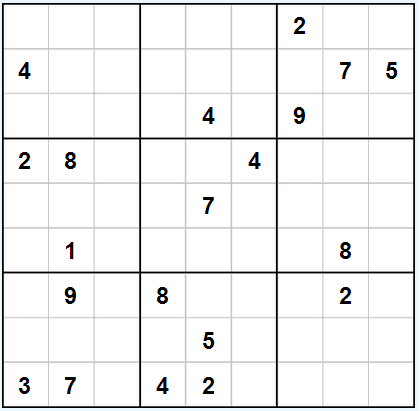
\includegraphics[scale=0.70]{sudoku.png}
        \caption{A standard $9$x$9$ sudoku puzzle.}
        \label{fig:sudoku}
    \end{figure}
    
    With the growing popularity of sudoku, many $9$x$9$ puzzles are required to feed the demand. Additionally, there is some demand
    for larger or smaller sudoku puzzles (rather than $9$x$9$) for a greater or simpler challenge.
    %\end{Sudoku}

%\end{Introduction}
